\section{Discussion} \label{sec:discussion}

Including the natural or potential local resource in estimates of total theoretical wave energy assessments -- as we propose here -- is a fundamental change in methodology. There are several practical questions about how this energy can be harnessed on both large and small scales. 
The potential local resource is particularly speculative because it only becomes available when large-scale wave energy extraction becomes economically feasible at great distance from shore. Even the natural local resource doesn't become a significant component of a wave energy project's resource until the size of the project is greater than several thousand square kilometers. As an example, consider fetch limited wave growth under a constant 10 m/s wind in deep water. Following \citet{donelan1980similarity} it will require 50 km of fetch for waves to have a modest wave flux of 1.5 kW/m. 

More work is needed to understand how much of the local resource overlaps with the offshore wind resource, and to identify what kinds of wave devices will efficiently harness the relatively high-frequency energy contained in the local resource. Though these questions and limitations exist, we still argue that including the local resource in the total theoretical resource is important for several reasons.

First, it is a real part of the total energy that is available -- or potentially available -- for conversion to electricity. Second, including it resolves outstanding questions associated with earlier resource assessments, thereby providing clarity to how regional wave resource assessments should be completed.  Third, including it broadens our understanding of what wave energy is; including it in our assessments gives a more complete picture of the opportunity. Fourth, and finally, the methodology proposed here -- which we have been applied at a regional scale -- can also be applied at the project scale to give an estimate of the theoretical resource at a site. This accuracy at all scales makes it ideally suited for broader adoption by the international community, which will in turn make the assessment of wave energy opportunities more comparable and transparent.

\subsection{The potential for wave energy in the U.S.}

The West Coast is typically viewed as the premier U.S. wave energy market because the resource and market are both large. The west coast's inner-shelf theoretical resource (410~TWh/yr) is equal to ~40\% of electricity consumption of California Oregon, and Washington (2018 total: 943 TWh/yr), which suggests that there is sufficient resource to play a sizable role in the region's energy profile \citep{energyinformationadministrationStateEnergyConsumption2020}.  
The fact that the remote wave energy resource here complements the offshore wind resource in several locations, suggests that OSW-wave hybrid projects might have higher annual capacity factors than projects involving one of these technologies alone. The PacWave test site, offshore of central Oregon, has been created to be the first U.S. "grid-connected full-scale test facility", which will provide the opportunity to develop and demonstrate technologies in this world-class ``fully energetic'' resource where winter storms can deliver wave amplitudes greater than 8 meters \citep[e.g.][]{allan_climate_2006}.

Though Alaska has a larger total resource than the West Coast, the majority of this is `stranded' -- very far from large populations where markets are large enough to attract projects bigger than a few MW. Still, the wave resource along Alaska's Aleutian chain is sizable, and raises the possibility of exporting the energy if and when large-scale energy storage technologies become sufficiently economical (e.g., renewable fuels, batteries, etc.). Could a breakthrough of this kind reignite Alaska's energy-export economy, this time for Alaska's vast renewable energy resources? In the shorter-term, the villages along Alaska's coastline -- where energy prices are very high -- represent an opportunity to demonstrate commercial viability before scaling the technology up \cite{alaskaenergyauthority2019PowerCost2020}. Or this energy could be used in-place for Blue Economy applications such as charging batteries on vessels or for scientific instruments during long transits or exploration. 

Hawaii possesses a relatively large resource (~430 TWh/yr total, 120 TWh/yr inner-shelf) considering the State's population and electricity consumption (26 TWh/yr), and is an especially attractive early market for wave energy because of the State's high-energy prices. 
Wave energy may be particularly valued in Hawaii where space is limited for land-based renewable alternatives; the tourist economy there may especially value WECs with limited surface expression. Together, these factors make Hawaii a likely early-market for wave energy technology. The Navy's Wave Energy Test Site on the north shore of Oahu, is supporting the development and demonstration of technologies for meeting the potential demand \citep{crossEarlyResearchEfforts2015}.

The East Coast and Gulf of Mexico wave resources are modest in comparison to the above regions. Still, it is too early to neglect the potential for wave energy in these regions. As wave technologies continues to mature and if the cost of the technology is low enough, sites and regions previously considered uneconomical may prove to be attractive, especially in markets where energy prices are already high and alternate renewable sources are limited or constrained. Small grids such as those in Puerto Rico, the U.S. Virgin Islands, and in remote Alaska are struggling to identify affordable and reliable local sources of power. Wave energy could help to fill periods of time when other sources of energy are unavailable (renewable or not), thereby increasing the resiliency of the grid-system.

\subsection{Predictability of wave energy}
One of the main advantages of wave energy is the idea that it is much more predictable than most other renewable energies. On daily to weekly timescales, wave can be predicted by wave propagation models driven be real-time earth observation data-sources (satellites, buoys, etc.).

On inter-annual timescales, several works have noted a correlation with ENSO fluctuations. Figure \ref{fig:wc-nino} compares the West Coast remote wave resource anomaly (the deviation from the annual mean) to the Oceanic Nino Index (ONI) lagged by 2 months. \cite{nationaloceanicandatmosphericadministrationOceanicNinoIndex2020}.
Here we see a strong correlation between the highest values of the west coast resource anomaly and high values of ONI. The fact that the wave resource lags the ONI suggests that the ONI can be used to predict peaks in wave energy. This correlation is likely to be causal because ENSO events are correlated with larger storms in the S. Pacific, which is a major source of wave energy on the U.S. West Coast \citep{andersonClimateIndexOptimized2018, yangCharacteristicsVariabilityNearshore2020, ruggieroNationalAssessmentShoreline2013}.

On shorter timescales, modern improvements in wave modeling have made significant advances in the accuracy of wave prediction \citep{cavaleriWaveModellingCoastal2018}. Applications of artificial intelligence have also shown promise for accurate prediction of wave height and wave power \citep[e.g.][]{cornejo-bueno_significant_2016}. This predictability, and the degree to which wave energy compliments other types of renewable energy in specific locations, may become increasingly valuable as electrical grids are powered increasingly by variable renewables \cite{parkinsonIntegratingOceanWave2015}.

\begin{figure}[ht]
  \centering
  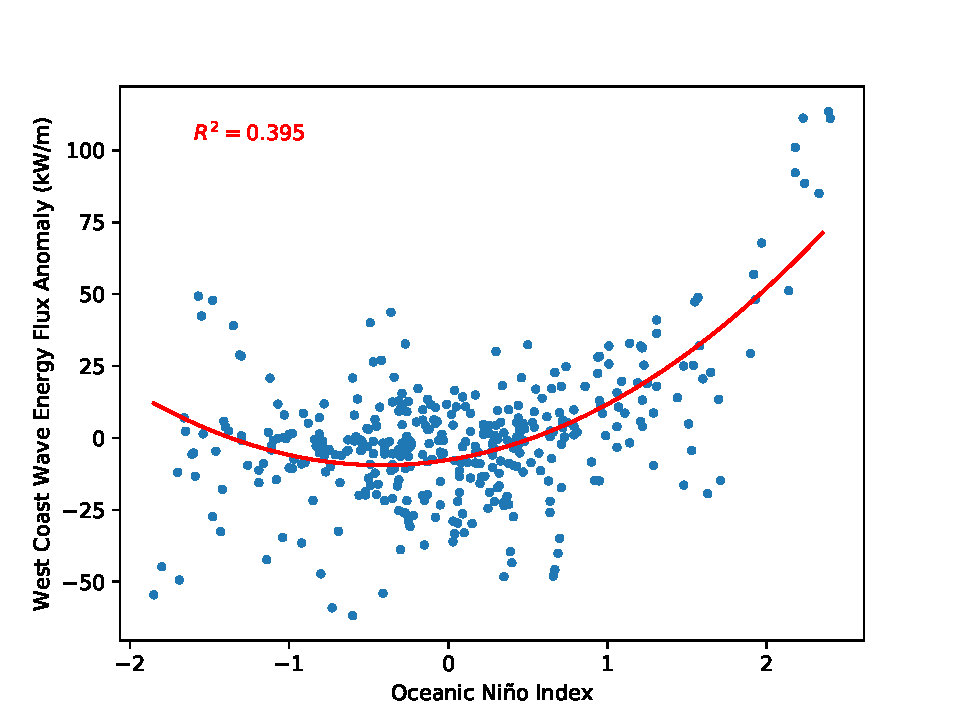
\includegraphics[width=\textwidth]{../fig/ENSO-Comparison.wc.pdf}
  \caption{West Coast wave energy flux anomaly vs. oceanic nino index. The wave energy flux anomaly (annual cycle removed) is averaged along the EEZ boundary, has had a 5-month running average applied, and lags the ONI signal by 2-months.}
  \label{fig:wc-nino}
\end{figure}


\section{Conclusion} \label{sec:conclusion}

We propose a methodology for theoretical wave resource assessment that resolves several outstanding issues with earlier approaches. In particular, this work accounts for wave directionality in order to reduce `double counting', and also includes the energy added to the wave field by local winds. This provides a consistent methodology for accounting for wave energy at national/regional scales. So that policy makers can have a clear understanding of wave energy potential. As other nations/regions adopt the methodology, we will have an apples-to-apples comparison of opportunity, which can inform decision making and investment.

We then apply this methodology to the U.S. EEZ (except for the portion of the EEZ associated with U.S. Pacific Islands Territories), and find that the total U.S. wave energy resource is greater than 3,300 TWh/yr.
This is an increase of ~25\% compared to earlier DOE wave resource assessments, and is due to the combination of extending the resource area to the edge of the EEZ and incorporating the local resource. The `inner shelf' resource (i.e., at 10 nautical-miles from shore) is estimated herein to be 1800 TWh/yr.

A detailed assessment of the ``technical resource potential'', which accounts for the efficiency and array design of existing technologies is left for future work. Furthermore, an assessment of the ``practical resource'' is a greater challenge because it requires accounting for regional permitting details, ocean-planning designations, and competing uses by other ocean stakeholders.

We encourage the IEC wave resource assessment team to consider adopting pieces of this methodology in the ``reconaissance'' level assessments in order to promote the adoption of consistent regional resource assessments methods. Furthermore, the methods proposed here could also be of use to project developers in identifying the maximum resource potential of a project site.

%\subsection{SOME EXTRA TEXT FROM DISCUSSION}

%Will devices of the future be sufficiently broad-banded to extract the local resource and remote resource equally efficiently? 
%What technological changes are required to make that happen? There is use for this energy in niche blue economy markets, or if energy storage technologies (e.g., liquid renewable fuels) become sufficiently inexpensive. If so, will the WEC technologies be economically competitive? 

%%% Local Variables:
%%% TeX-master: "wave_res"
%%% End:
